\chapter{Introduction}
\label{ch:introduction}

\section{Background and Motivation}
\label{sec:bg_motivation}

\subsection{Cryptography and the Need for Secure Communication}
In the modern digital era, the security of information transmission over public networks has become paramount. With the exponential growth of electronic commerce, wireless mobile communications, and cloud computing, sensitive personal, financial, and military data are constantly exposed to eavesdropping and active interception. Cryptography serves as the mathematical foundation for ensuring data confidentiality, integrity, authenticity, and non-repudiation. 

The primary objective of encryption is to transform intelligible plaintext into unintelligible ciphertext using a secret key. Without the key, recovering the plaintext must be computationally infeasible. Modern cryptography is broadly categorized into symmetric (secret-key) and asymmetric (public-key) cryptosystems. While public-key systems are indispensable for key exchange and digital signatures, symmetric-key systems remain the workhorse for high-speed bulk data encryption due to their computational efficiency.

\subsection{Symmetric Key Cryptography: Block Ciphers vs. Stream Ciphers}
Symmetric cryptosystems are split into two primary architectures: block ciphers and stream ciphers. 
\begin{itemize}
    \item \textbf{Block Ciphers:} Process the plaintext in fixed-size blocks (typically 64 or 128 bits) using a complex, iterative substitution-permutation network (SPN) or Feistel structure (e.g., AES, DES).
    \item \textbf{Stream Ciphers:} Encrypt plaintext digits (typically single bits) individually by combining them with a time-varying pseudorandom sequence called the \textit{keystream} (e.g., RC4, A5/1, E0). The combining operation is usually a simple bitwise exclusive-OR (XOR) addition.
\end{itemize}

A comparison of their characteristics is summarized in Table~\ref{tab:block_vs_stream}.

\begin{table}[h]
\centering
\caption{Comparison of Block Ciphers and Stream Ciphers}
\label{tab:block_vs_stream}
\begin{tabular}{@{}lll@{}}
\toprule
\textbf{Property} & \textbf{Block Ciphers} & \textbf{Stream Ciphers} \\ \midrule
\textbf{Granularity} & Fixed blocks (64/128 bits) & Bit-by-bit or byte-by-byte \\
\textbf{Encryption Speed} & Moderate (higher latency) & Very high (real-time processing) \\
\textbf{Hardware Complexity} & High (requires buffering) & Low (minimum gate count) \\
\textbf{Error Propagation} & Errors propagate across block & No propagation (single bit affected) \\
\textbf{State Synchronization} & Not required & Critical for synchronous ciphers \\
\textbf{Primary Domain} & File storage, web protocols & Wireless channels, embedded systems \\ \bottomrule
\end{tabular}
\end{table}

\subsection{Role of Stream Ciphers in Modern Security Systems}
Stream ciphers are preferred in resource-constrained environments where memory, processing power, and battery capacity are limited, or where latency must be strictly minimized. By reducing the complex diffusion-confusion operations of block ciphers into a stateful pseudorandom number generator (PRNG) that produces a keystream, stream ciphers can achieve extremely high throughput in hardware with very low gate counts. Furthermore, the absence of error propagation makes stream ciphers highly suitable for noisy wireless communication channels where single-bit transmission errors should not corrupt subsequent data blocks.

\subsection{Why Stream Cipher Security Matters — Real-World Applications}
The security of stream ciphers directly impacts several legacy and contemporary communication protocols:
\begin{itemize}
    \item \textbf{GSM (A5/1, A5/2):} Used to secure voice communication in 2G cellular networks. A5/1 relies on three irregularly clocked LFSRs.
    \item \textbf{Bluetooth (E0):} Encrypts packets over the air using a combining generator with four LFSRs and a 16-state machine.
    \item \textbf{Wi-Fi (RC4 in WEP/WPA):} Historically secured wireless networks, though RC4 is a software-oriented byte-based cipher rather than an LFSR-based design.
\end{itemize}
Understanding the vulnerabilities of these ciphers under advanced cryptanalytic attacks is essential for designing modern, quantum-resistant stream ciphers (such as the eSTREAM portfolio designs like Grain and Trivium).

\section{Stream Cipher Fundamentals}
\label{sec:stream_fundamentals}

\subsection{Keystream Generation Model}
A synchronous stream cipher consists of a state space $\mathcal{X}$, an initialization vector (IV), a secret key $K$, a state transition function $g: \mathcal{X} \to \mathcal{X}$, and an output function $h: \mathcal{X} \to \mathbb{F}_2$. The internal state $S_t$ at time $t$ evolves as:
$$S_{t+1} = g(S_t)$$
The keystream bit $y_t$ is generated by:
$$y_t = h(S_t)$$
The ciphertext $c_t$ is computed via:
$$c_t = p_t \oplus y_t$$
where $p_t$ is the plaintext bit. Decryption is identical: $p_t = c_t \oplus y_t$.

\subsection{Synchronous vs. Self-Synchronizing Stream Ciphers}
Stream ciphers are divided into two main categories:
\begin{enumerate}
    \item \textbf{Synchronous Stream Ciphers:} The keystream is generated independently of the plaintext and ciphertext. Sender and receiver must remain in exact state synchronization. If a bit is lost during transmission, synchronization is broken, and decryption fails until a resynchronization protocol is executed.
    \item \textbf{Self-Synchronizing (Asynchronous) Stream Ciphers:} The keystream depends on a fixed window of previous ciphertext bits. If a ciphertext bit is corrupted or lost, the error propagates only for the length of the shift register window, after which the system automatically self-synchronizes.
\end{enumerate}
Our proposed attack targets the synchronous stream cipher model.

\subsection{Security Requirements for Stream Ciphers}
For a stream cipher to be cryptographically secure, the keystream $y_t$ must possess the following properties:
\begin{itemize}
    \item \textbf{Large Period:} The period $T$ of the sequence must be sufficiently large ($T > 2^{80}$) to prevent keystream reuse.
    \item \textbf{High Linear Complexity:} The linear complexity $LC$ must be large ($LC > T/2$) to prevent state recovery using the Berlekamp-Massey algorithm.
    \item \textbf{Randomness Properties:} The keystream must satisfy Golomb's three randomness postulates:
    \begin{enumerate}
        \item \textit{Balance property:} The number of zeros and ones in a period differs by at most 1.
        \item \textit{Run property:} Runs of consecutive identical bits decrease exponentially in frequency.
        \item \textit{Autocorrelation property:} The out-of-phase autocorrelation is constant.
    \end{enumerate}
\end{itemize}

\section{Linear Feedback Shift Registers (LFSRs)}
\label{sec:lfsrs}

\subsection{Definition and Mathematical Representation}
A Linear Feedback Shift Register (LFSR) of length $L$ consists of $L$ stages (flip-flops) storing state bits $s_0, s_1, \dots, s_{L-1}$ and a feedback tap coefficient vector $(c_1, c_2, \dots, c_L) \in \mathbb{F}_2^L$. At each clock cycle, the register is shifted, and the new leftmost bit is computed as a linear combination of the current state:
$$s_{t+L} = c_1 s_{t+L-1} \oplus c_2 s_{t+L-2} \oplus \dots \oplus c_L s_t = \sum_{i=1}^L c_i s_{t+L-i} \pmod{2}$$
with $c_L = 1$ to ensure the recurrence is of degree $L$.

\begin{figure}[h]
\centering
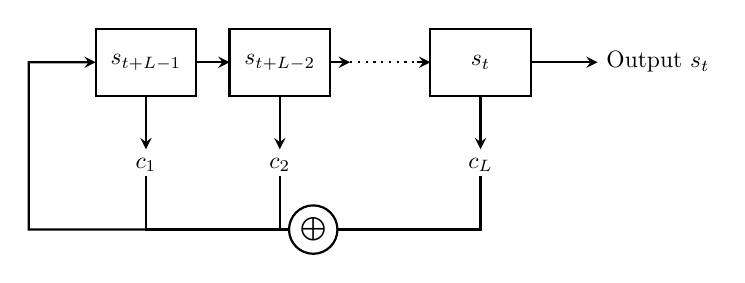
\begin{tikzpicture}[scale=0.85, every node/.style={transform shape}]
    % Shift Register Blocks
    \draw[thick] (0,0) rectangle (1.5,1) node[pos=0.5] {$s_{t+L-1}$};
    \draw[thick] (2,0) rectangle (3.5,1) node[pos=0.5] {$s_{t+L-2}$};
    \draw[dotted, thick] (3.8,0.5) -- (4.8,0.5);
    \draw[thick] (5,0) rectangle (6.5,1) node[pos=0.5] {$s_t$};
    
    % Shift arrows
    \draw[->, >=stealth, thick] (1.5,0.5) -- (2,0.5);
    \draw[->, >=stealth, thick] (3.5,0.5) -- (3.8,0.5);
    \draw[->, >=stealth, thick] (4.8,0.5) -- (5,0.5);
    \draw[->, >=stealth, thick] (6.5,0.5) -- (7.5,0.5) node[right] {Output $s_t$};
    
    % Feedback taps
    \draw[->, >=stealth, thick] (0.75,0) -- (0.75,-0.8) node[below] {$c_1$};
    \draw[->, >=stealth, thick] (2.75,0) -- (2.75,-0.8) node[below] {$c_2$};
    \draw[->, >=stealth, thick] (5.75,0) -- (5.75,-0.8) node[below] {$c_L$};
    
    % Feedback sum
    \node[draw, circle, thick, inner sep=2pt] (sum) at (3.25,-2) {$\bigoplus$};
    
    \draw[thick] (0.75,-1.2) |- (sum);
    \draw[thick] (2.75,-1.2) |- (sum);
    \draw[thick] (5.75,-1.2) |- (sum);
    
    % Feedback loop connection
    \draw[->, >=stealth, thick] (sum.west) -- (-1,-2) -- (-1,0.5) -- (0,0.5);
\end{tikzpicture}
\caption{Feedback Loop and Shift Stages of a Linear Feedback Shift Register (LFSR)}
\label{fig:lfsr_fibonacci}
\end{figure}

\subsection{Feedback Polynomials and Primitive Polynomials}
The behavior of the shift register sequence is governed by its characteristic feedback polynomial:
$$C(x) = x^L \oplus c_1 x^{L-1} \oplus c_2 x^{L-2} \oplus \dots \oplus c_L \in \mathbb{F}_2[x]$$
To achieve the maximum possible period of $T = 2^L - 1$ (making the output sequence an $m$-sequence), $C(x)$ must be a \textit{primitive polynomial} over $\mathbb{F}_2$. A polynomial is primitive if it is irreducible and the smallest integer $k$ for which $C(x)$ divides $x^k - 1$ is $k = 2^L - 1$.

\subsection{State Transition and the Companion Matrix}
The state of the LFSR at time $t$ can be represented as a vector $\mathbf{S}_t = [s_t, s_{t+1}, \dots, s_{t+L-1}]^T$. The transition to the next state is represented by a linear transformation:
$$\mathbf{S}_{t+1} = \mathbf{M} \cdot \mathbf{S}_t$$
where $\mathbf{M}$ is the $L \times L$ Companion Matrix over $\mathbb{F}_2$:
$$\mathbf{M} = \begin{pmatrix}
0 & 1 & 0 & \dots & 0 \\
0 & 0 & 1 & \dots & 0 \\
\vdots & \vdots & \vdots & \ddots & \vdots \\
0 & 0 & 0 & \dots & 1 \\
c_L & c_{L-1} & c_{L-2} & \dots & c_1
\end{pmatrix}$$
By induction, the state at any time $t$ is given by:
$$\mathbf{S}_t = \mathbf{M}^t \cdot \mathbf{S}_0$$
This linear structure means the entire output sequence is uniquely determined by the initial seed vector $\mathbf{S}_0$.

\subsection{Properties of $m$-sequences}
Maximal-length sequences ($m$-sequences) produced by primitive polynomials satisfy Golomb's randomness criteria:
1.  \textbf{Balance:} The period contains $2^{L-1}$ ones and $2^{L-1}-1$ zeros.
2.  \textbf{Autocorrelation:} The autocorrelation function $R(\tau)$ is:
    $$R(\tau) = \begin{cases}
    1, & \text{if } \tau \equiv 0 \pmod{2^L-1} \\
    -\frac{1}{2^L-1}, & \text{otherwise}
    \end{cases}$$

\subsection{Why LFSRs Alone Are Insecure — The Berlekamp–Massey Attack}
Despite their excellent statistical properties, LFSRs are cryptographically weak when used alone. Because the feedback relation is linear, observing only $2L$ consecutive keystream bits allows an attacker to construct a system of $L$ linear equations in $L$ unknowns. This system can be solved in $O(L^2)$ operations using the **Berlekamp-Massey Algorithm** to reconstruct the feedback polynomial $C(x)$ and the initial state. Thus, to build a secure stream cipher, nonlinear components must be introduced.

\section{Combining Function Generators}
\label{sec:combining_generators}

\subsection{Nonlinear Combining of Multiple LFSRs}
To destroy the linearity of individual LFSR sequences, a combining generator runs $k$ parallel LFSRs, each initialized with a secret seed. The outputs $x_1^{(t)}, x_2^{(t)}, \dots, x_k^{(t)}$ are combined using a nonlinear Boolean function $f(x_1, x_2, \dots, x_k)$ to generate the keystream $y_t$:
$$y_t = f(x_1^{(t)}, x_2^{(t)}, \dots, x_k^{(t)})$$

\begin{figure}[h]
\centering
\begin{tikzpicture}[scale=0.9, every node/.style={transform shape}]
    % LFSR blocks
    \draw[thick] (0, 2) rectangle (2, 2.8) node[pos=0.5] {$\text{LFSR}_1$};
    \draw[thick] (0, 0.8) rectangle (2, 1.6) node[pos=0.5] {$\text{LFSR}_2$};
    \node at (1, 0.2) {$\vdots$};
    \draw[thick] (0, -1.2) rectangle (2, -0.4) node[pos=0.5] {$\text{LFSR}_k$};
    
    % Combining function box
    \draw[thick, fill=lightblue] (4, -0.8) rectangle (6, 2.4) node[pos=0.5, align=center] {Combining\\Function\\$f(x_1, \dots, x_k)$};
    
    % Input lines
    \draw[->, >=stealth, thick] (2, 2.4) -- (4, 2.4) node[midway, above] {$x_1^{(t)}$};
    \draw[->, >=stealth, thick] (2, 1.2) -- (4, 1.2) node[midway, above] {$x_2^{(t)}$};
    \draw[->, >=stealth, thick] (2, -0.8) -- (4, -0.8) node[midway, above] {$x_k^{(t)}$};
    
    % Output line
    \draw[->, >=stealth, thick] (6, 0.8) -- (7.5, 0.8) node[right] {Keystream $y_t$};
\end{tikzpicture}
\caption{Architecture of a Nonlinear Combining Generator}
\label{fig:combining_generator}
\end{figure}

\subsection{Boolean Functions: ANF and Algebraic Degree}
Any Boolean function $f: \mathbb{F}_2^k \to \mathbb{F}_2$ can be uniquely represented in its **Algebraic Normal Form (ANF)** as a multivariate polynomial over $\mathbb{F}_2$:
$$f(x_1, \dots, x_k) = a_0 \oplus \bigoplus_{i=1}^k a_i x_i \oplus \bigoplus_{1 \le i < j \le k} a_{ij} x_i x_j \oplus \dots \oplus a_{12\dots k} x_1 x_2 \dots x_k$$
The **algebraic degree** $d$ of $f$ is the maximum number of variables in any product term with a non-zero coefficient $a_{i_1\dots i_r}$. To prevent algebraic reduction attacks, the combining function must have a high algebraic degree.

\subsection{Correlation Immunity and Resilience (Siegenthaler's Bound)}
A Boolean function is $t$th-order **correlation-immune** if the output $y = f(x_1, \dots, x_k)$ is statistically independent of any subset of $t$ input variables. If the function is also balanced, it is called $t$-resilient.

In 1984, Siegenthaler proved a fundamental trade-off between the algebraic degree $d$ and the correlation immunity order $t$ of a function:
$$d + t \le k$$
For a balanced function, the bound is stricter:
$$d + t \le k - 1 \quad (\text{for } t \ge 1)$$
This bound presents a dilemma: maximizing resistance to algebraic attacks (high $d$) weakens resistance to correlation attacks (low $t$), and vice versa.

\subsection{Nonlinearity and the Walsh Spectrum}
The Walsh-Hadamard Transform (WHT) of a Boolean function $f(x)$ represents its correlation with all linear functions. Let $\chi_u(x) = (-1)^{u \cdot x}$ be a character function, where $u \cdot x = \sum u_i x_i \pmod{2}$. The Walsh transform of the sign function $\hat{f}(x) = (-1)^{f(x)}$ is defined as:
$$\hat{F}(u) = \sum_{x \in \mathbb{F}_2^k} (-1)^{f(x) \oplus u \cdot x}$$
The nonlinearity $\mathcal{NL}(f)$ of the function is related to its maximum Walsh coefficient:
$$\mathcal{NL}(f) = 2^{k-1} - \frac{1}{2} \max_{u \in \mathbb{F}_2^k} |\hat{F}(u)|$$
A low maximum Walsh coefficient implies high nonlinearity, protecting the cipher against linear cryptanalysis.

\subsection{The Majority Function ($p = 0.75$)}
For a 3-input combining generator, the standard majority function is:
$$f(x_1, x_2, x_3) = \text{Threshold}_2(x_1, x_2, x_3) = x_1 x_2 \oplus x_2 x_3 \oplus x_3 x_1$$
The majority function is balanced and has algebraic degree $d=2$. However, its correlation immunity is $t=0$, meaning its output is correlated with its inputs. Specifically, the probability that the output equals any individual input is:
$$P(f(x_1, x_2, x_3) = x_i) = 0.75 \quad (p = 0.75)$$
This statistical leakage of $p = 0.75$ ($\epsilon = 0.50$) is exploited by correlation attacks.

\subsection{The Geffe Generator}
The Geffe generator combines three LFSRs using the multiplexing function:
$$f(x_1, x_2, x_3) = x_1 x_2 \oplus (1 \oplus x_1) x_3$$
where $\text{LFSR}_1$ acts as a selector control.
- If $x_1 = 1$, the output is $x_2$.
- If $x_1 = 0$, the output is $x_3$.
The correlation probabilities are:
$$P(f = x_1) = 0.50 \quad (\text{correlation-immune})$$
$$P(f = x_2) = P(f = x_3) = 0.75 \quad (\text{bias } \epsilon = 0.50)$$
This asymmetry allows an attacker to target $\text{LFSR}_2$ and $\text{LFSR}_3$ independently, recovering their states before solving for the selector register $\text{LFSR}_1$.

\section{Cryptanalytic Attack Models}
\label{sec:attack_models}

\subsection{Ciphertext-Only, Known-Plaintext, and Chosen-Plaintext Attacks}
Cryptanalytic attacks are evaluated based on the attacker's capabilities:
1.  \textbf{Ciphertext-Only Attack (COA):} The attacker only observes the ciphertext. For stream ciphers, this is often sufficient if the plaintext has redundancy.
2.  \textbf{Known-Plaintext Attack (KPA):} The attacker has access to corresponding pairs of plaintext and ciphertext. Since $y_t = p_t \oplus c_t$, a KPA gives the attacker direct access to $N$ consecutive keystream bits. This is the standard model used to evaluate correlation attacks.
3.  \textbf{Chosen-Plaintext Attack (CPA):} The attacker can choose plaintext inputs and observe the ciphertexts.

Our work assumes the **Known-Plaintext Attack (KPA)** model.

\subsection{Divide-and-Conquer Attacks on Combining Generators}
The core weakness of combining generators is their susceptibility to divide-and-conquer strategies. Instead of searching the joint key space of size $2^{L_1 + L_2 + L_3}$, the correlation leakage $P(y_t = x_i^{(t)}) = p > 0.5$ allows the attacker to isolate and attack each register independently. The search space is reduced to:
$$\sum_{i=1}^k 2^{L_i} \ll \prod_{i=1}^k 2^{L_i}$$
For a $3 \times 25$-bit generator, the search complexity is reduced from $2^{75} \approx 3.77 \times 10^{22}$ tests to $3 \times 2^{25} \approx 10^8$ tests, which is computationally practical.

\subsection{Taxonomy of Attacks on LFSR-Based Stream Ciphers}
- **Correlation Attacks (Siegenthaler, 1985):** Naive exhaustive correlation search over $2^L$ seeds per LFSR.
- **Fast Correlation Attacks (FCA) (Meier-Staffelbach, 1989):** Translates the search into a decoding problem over a Binary Symmetric Channel (BSC), using parity-check equations to correct keystream errors.
- **Algebraic Attacks:** Sets up systems of nonlinear multivariate equations representing the state transitions and solves them using Gröbner bases or linearization.
- **Time-Memory-Data Trade-off (TMDTO) Attacks:** Exploits state space collisions using precomputed tables to trade off online attack time for memory storage.

\section{Problem Statement}
\label{sec:problem_statement}

\subsection{The Gap Between Exhaustive Correlation and Fast Correlation Attacks}
In the cryptanalysis of combining ciphers, there is a clear trade-off between the standard correlation attack and fast correlation attacks:
- **Exhaustive Correlation** has a high computational complexity of $O(N \cdot 2^L)$ per register. However, it is mathematically robust and guaranteed to succeed given sufficient keystream, regardless of the feedback polynomial's structure.
- **Fast Correlation Attacks (FCA)** have sub-exponential time complexity but are highly dependent on the existence of low-weight parity-check equations. For ciphers with dense feedback polynomials or large register lengths $L \ge 25$, finding low-weight multiples within short keystream boundaries is often impossible, causing FCA success rates to drop to $0\%$.

\subsection{Limitations of Existing WHT Approaches}
While Chose, Joux, and Mitton (2002) proposed using the Walsh-Hadamard Transform for bulk correlation computation, their design processed the entire keystream $N$ in the spectral accumulator. This resulted in an $O(N \cdot L + L \cdot 2^L)$ time complexity, which does not scale efficiently for long keystreams. There is no existing method that utilizes WHT on a partial keystream prefix to prune the search space prior to precise correlation.

\section{Research Objectives and Contributions}
\label{sec:objectives}
This thesis addresses the cryptanalytic gap by introducing a two-stage cascade correlation attack accelerated by the Walsh-Hadamard Transform. The primary contributions of this work are:
\begin{enumerate}
    \item \textbf{Algorithmic Design:} We propose the \textbf{Two-Stage Cascade WHT Attack} that limits the expensive WHT computation to a short prefix $N_1 \ll N$, pruning the search space to a candidate pool of size $M = \sqrt{2^L}$. The full keystream $N$ is only processed on the survivors, reducing complexity to $O(L \cdot 2^L + \sqrt{2^L} \cdot N)$.
    \item \textbf{Mathematical Rigor:} We prove the \textbf{Pruning Survival Theorem}, utilizing Central Limit Theorem approximations and extreme value order statistics to derive a closed-form equation for the survival probability of the correct seed.
    \item \textbf{Parameter Optimization:} We establish an adaptive parameter-selection method (\texttt{compute\_optimal\_n1}) that guarantees a $99\%$ survival probability of the correct seed for any configuration $(L, M, p)$.
    \item \textbf{Research-Scale Validation:} We benchmark the attack on a 75-bit key Combining Generator ($L = 25$ registers) compiled with Numba JIT. Our results show a \textbf{102$\times$ speedup} over standard exhaustive correlation, while Meier-Staffelbach FCA fails completely.
\end{enumerate}

\section{Organisation of the Report}
\label{sec:organisation}
The remainder of this report is organized as follows:
\begin{itemize}
    \item \textbf{Chapter 2 (Literature Survey):} Reviews the theoretical foundations of correlation attacks, fast correlation attacks, and mathematical formulations of the WHT in cryptanalysis.
    \item \textbf{Chapter 3 (Proposed Attack):} Details the mathematical foundation, the two-stage cascade architecture, and the proof of the Pruning Survival Theorem.
    \item \textbf{Chapter 4 (Research Analysis):} Presents the experimental results, timing breakdowns, parameter sweeps, and Monte Carlo validations.
    \item \textbf{Chapter 5 (Conclusion \& Future Scope):} Summarizes the contributions, discusses the practical scalability limits (the Memory Wall), and outlines future research avenues.
\end{itemize}
